\documentclass{standalone}
\usepackage{tikz}
\usetikzlibrary{patterns, positioning}


\begin{document}
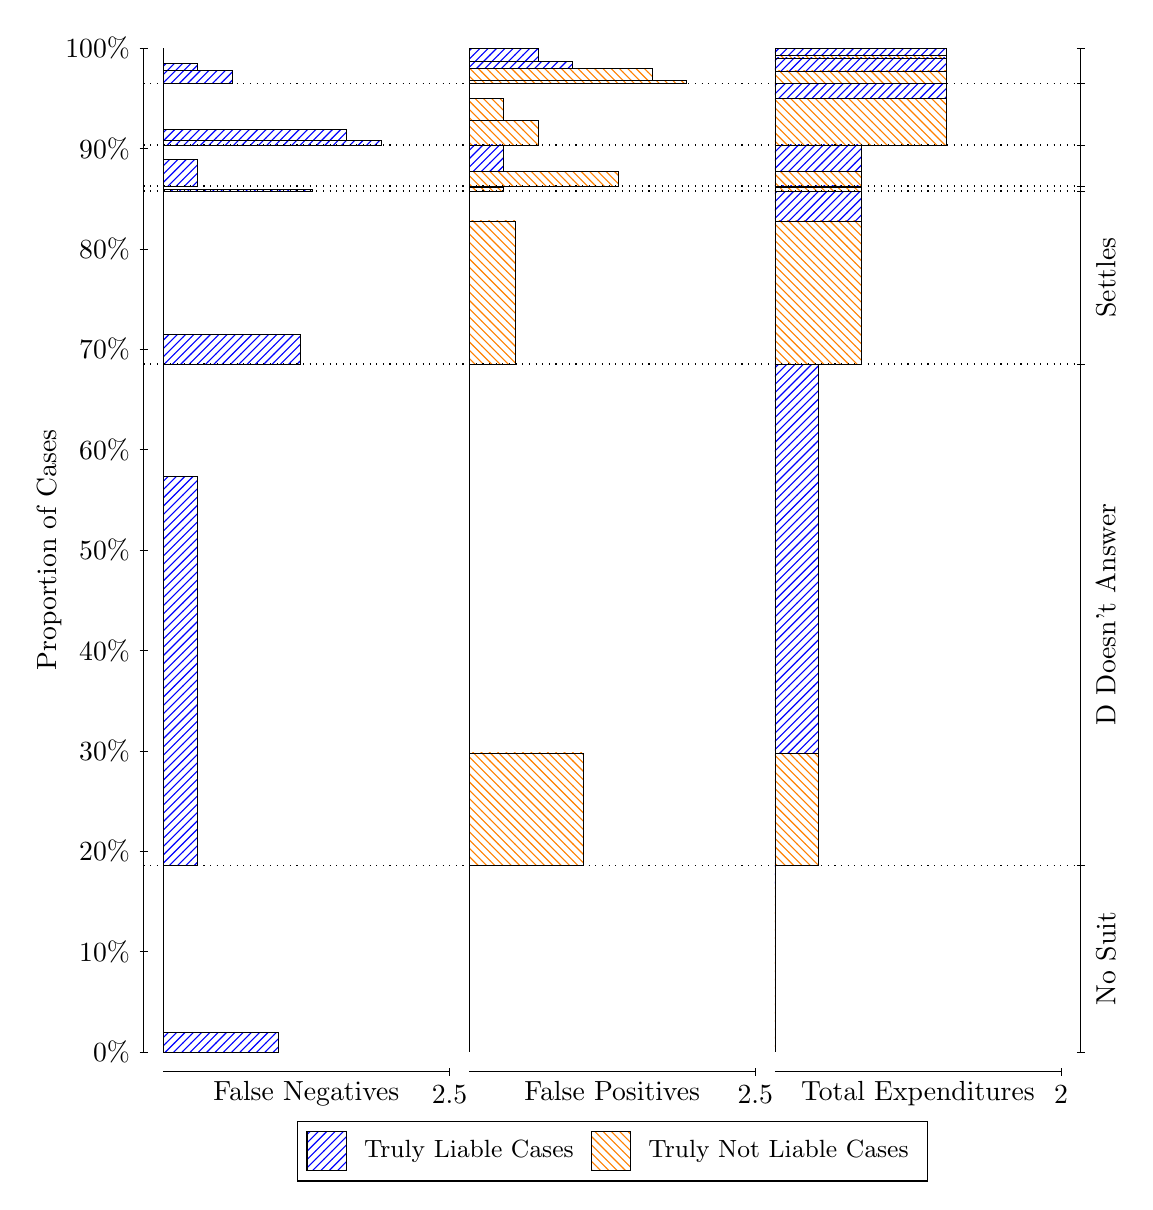
\begin{tikzpicture}
\draw[black, very thin] (1.5,1.75) -- (1.5,14.5);
\node[rotate=90, text=black, anchor=center] at (0.3, 8.125) {Proportion of Cases};
\draw[black, very thin] (1.45,1.75) -- (1.55,1.75);
\node[text=black, anchor=east] at (1.45, 1.75) {0\%};
\draw[black, very thin] (1.45,3.025) -- (1.55,3.025);
\node[text=black, anchor=east] at (1.45, 3.025) {10\%};
\draw[black, very thin] (1.45,4.3) -- (1.55,4.3);
\node[text=black, anchor=east] at (1.45, 4.3) {20\%};
\draw[black, very thin] (1.45,5.575) -- (1.55,5.575);
\node[text=black, anchor=east] at (1.45, 5.575) {30\%};
\draw[black, very thin] (1.45,6.85) -- (1.55,6.85);
\node[text=black, anchor=east] at (1.45, 6.85) {40\%};
\draw[black, very thin] (1.45,8.125) -- (1.55,8.125);
\node[text=black, anchor=east] at (1.45, 8.125) {50\%};
\draw[black, very thin] (1.45,9.4) -- (1.55,9.4);
\node[text=black, anchor=east] at (1.45, 9.4) {60\%};
\draw[black, very thin] (1.45,10.675) -- (1.55,10.675);
\node[text=black, anchor=east] at (1.45, 10.675) {70\%};
\draw[black, very thin] (1.45,11.95) -- (1.55,11.95);
\node[text=black, anchor=east] at (1.45, 11.95) {80\%};
\draw[black, very thin] (1.45,13.225) -- (1.55,13.225);
\node[text=black, anchor=east] at (1.45, 13.225) {90\%};
\draw[black, very thin] (1.45,14.5) -- (1.55,14.5);
\node[text=black, anchor=east] at (1.45, 14.5) {100\%};

\draw[black, very thin] (13.4,1.75) -- (13.4,14.5);
\draw[black, very thin] (13.35,1.75) -- (13.45,1.75);
\node[anchor=west] at (13.35, 1.75) {};
\draw[black, very thin] (13.35,4.1224) -- (13.45,4.1224);
\node[anchor=west] at (13.35, 4.1224) {};
\draw[black, very thin] (13.35,10.487) -- (13.45,10.487);
\node[anchor=west] at (13.35, 10.487) {};
\draw[black, very thin] (13.35,12.684) -- (13.45,12.684);
\node[anchor=west] at (13.35, 12.684) {};
\draw[black, very thin] (13.35,12.748) -- (13.45,12.748);
\node[anchor=west] at (13.35, 12.748) {};
\draw[black, very thin] (13.35,13.269) -- (13.45,13.269);
\node[anchor=west] at (13.35, 13.269) {};
\draw[black, very thin] (13.35,14.052) -- (13.45,14.052);
\node[anchor=west] at (13.35, 14.052) {};
\draw[black, very thin] (13.35,14.5) -- (13.45,14.5);
\node[anchor=west] at (13.35, 14.5) {};

\draw[black, very thin, pattern color=blue, pattern=north east lines] (1.75,1.75) rectangle (3.2033,1.9996);
\draw[black, very thin, pattern color=orange, pattern=north west lines] (1.75,1.9996) rectangle (1.75,4.1224);
\draw[black, very thin, pattern color=blue, pattern=north east lines] (1.75,4.1224) rectangle (2.186,9.0609);
\draw[black, very thin, pattern color=orange, pattern=north west lines] (1.75,9.0609) rectangle (1.75,10.487);
\draw[black, very thin, pattern color=blue, pattern=north east lines] (1.75,10.487) rectangle (3.494,10.866);
\draw[black, very thin, pattern color=orange, pattern=north west lines] (1.75,10.866) rectangle (1.75,12.684);
\draw[black, very thin, pattern color=blue, pattern=north east lines] (1.75,12.684) rectangle (3.6393,12.703);
\draw[black, very thin, pattern color=orange, pattern=north west lines] (1.75,12.703) rectangle (1.75,12.748);
\draw[black, very thin, pattern color=blue, pattern=north east lines] (1.75,12.748) rectangle (2.186,13.088);
\draw[black, very thin, pattern color=orange, pattern=north west lines] (1.75,13.088) rectangle (1.75,13.269);
\draw[black, very thin, pattern color=blue, pattern=north east lines] (1.75,13.269) rectangle (4.5113,13.323);
\draw[black, very thin, pattern color=blue, pattern=north east lines] (1.75,13.323) rectangle (4.0753,13.463);
\draw[black, very thin, pattern color=orange, pattern=north west lines] (1.75,13.463) rectangle (1.75,14.052);
\draw[black, very thin, pattern color=blue, pattern=north east lines] (1.75,14.052) rectangle (2.622,14.217);
\draw[black, very thin, pattern color=blue, pattern=north east lines] (1.75,14.217) rectangle (2.186,14.307);
\draw[black, very thin, pattern color=orange, pattern=north west lines] (1.75,14.307) rectangle (1.75,14.5);
\draw[black, very thin, pattern color=orange, pattern=north west lines] (5.6333,1.75) rectangle (5.6333,3.8728);
\draw[black, very thin, pattern color=blue, pattern=north east lines] (5.6333,3.8728) rectangle (5.6333,4.1224);
\draw[black, very thin, pattern color=orange, pattern=north west lines] (5.6333,4.1224) rectangle (7.0867,5.5484);
\draw[black, very thin, pattern color=blue, pattern=north east lines] (5.6333,5.5484) rectangle (5.6333,10.487);
\draw[black, very thin, pattern color=orange, pattern=north west lines] (5.6333,10.487) rectangle (6.2147,12.305);
\draw[black, very thin, pattern color=blue, pattern=north east lines] (5.6333,12.305) rectangle (5.6333,12.684);
\draw[black, very thin, pattern color=orange, pattern=north west lines] (5.6333,12.684) rectangle (6.0693,12.729);
\draw[black, very thin, pattern color=blue, pattern=north east lines] (5.6333,12.729) rectangle (5.6333,12.748);
\draw[black, very thin, pattern color=orange, pattern=north west lines] (5.6333,12.748) rectangle (7.5227,12.929);
\draw[black, very thin, pattern color=blue, pattern=north east lines] (5.6333,12.929) rectangle (6.0693,13.269);
\draw[black, very thin, pattern color=orange, pattern=north west lines] (5.6333,13.269) rectangle (6.5053,13.581);
\draw[black, very thin, pattern color=orange, pattern=north west lines] (5.6333,13.581) rectangle (6.0693,13.858);
\draw[black, very thin, pattern color=blue, pattern=north east lines] (5.6333,13.858) rectangle (5.6333,14.052);
\draw[black, very thin, pattern color=orange, pattern=north west lines] (5.6333,14.052) rectangle (8.3947,14.088);
\draw[black, very thin, pattern color=orange, pattern=north west lines] (5.6333,14.088) rectangle (7.9587,14.245);
\draw[black, very thin, pattern color=blue, pattern=north east lines] (5.6333,14.245) rectangle (6.9413,14.335);
\draw[black, very thin, pattern color=blue, pattern=north east lines] (5.6333,14.335) rectangle (6.5053,14.5);
\draw[black, very thin, pattern color=orange, pattern=north west lines] (9.5167,1.75) rectangle (9.5167,3.8728);
\draw[black, very thin, pattern color=blue, pattern=north east lines] (9.5167,3.8728) rectangle (9.5167,4.1224);
\draw[black, very thin, pattern color=orange, pattern=north west lines] (9.5167,4.1224) rectangle (10.062,5.5484);
\draw[black, very thin, pattern color=blue, pattern=north east lines] (9.5167,5.5484) rectangle (10.062,10.487);
\draw[black, very thin, pattern color=orange, pattern=north west lines] (9.5167,10.487) rectangle (10.607,12.305);
\draw[black, very thin, pattern color=blue, pattern=north east lines] (9.5167,12.305) rectangle (10.607,12.684);
\draw[black, very thin, pattern color=orange, pattern=north west lines] (9.5167,12.684) rectangle (10.607,12.729);
\draw[black, very thin, pattern color=blue, pattern=north east lines] (9.5167,12.729) rectangle (10.607,12.748);
\draw[black, very thin, pattern color=orange, pattern=north west lines] (9.5167,12.748) rectangle (10.607,12.929);
\draw[black, very thin, pattern color=blue, pattern=north east lines] (9.5167,12.929) rectangle (10.607,13.269);
\draw[black, very thin, pattern color=orange, pattern=north west lines] (9.5167,13.269) rectangle (11.697,13.858);
\draw[black, very thin, pattern color=blue, pattern=north east lines] (9.5167,13.858) rectangle (11.697,14.052);
\draw[black, very thin, pattern color=orange, pattern=north west lines] (9.5167,14.052) rectangle (11.697,14.209);
\draw[black, very thin, pattern color=blue, pattern=north east lines] (9.5167,14.209) rectangle (11.697,14.374);
\draw[black, very thin, pattern color=orange, pattern=north west lines] (9.5167,14.374) rectangle (11.697,14.41);
\draw[black, very thin, pattern color=blue, pattern=north east lines] (9.5167,14.41) rectangle (11.697,14.5);
\draw[black, dotted] (1.5,4.1224) -- (13.4,4.1224);
\draw[black, dotted] (1.5,10.487) -- (13.4,10.487);
\draw[black, dotted] (1.5,12.684) -- (13.4,12.684);
\draw[black, dotted] (1.5,12.748) -- (13.4,12.748);
\draw[black, dotted] (1.5,13.269) -- (13.4,13.269);
\draw[black, dotted] (1.5,14.052) -- (13.4,14.052);
\draw[black, very thin] (1.75,1.5) -- (5.3833,1.5);
\node[text=black, anchor=north] at (3.5667, 1.5) {False Negatives};
\draw[black, very thin] (5.3833,1.45) -- (5.3833,1.55);
\node[text=black, anchor=north] at (5.3833, 1.45) {2.5};

\draw[black, very thin] (5.6333,1.5) -- (9.2667,1.5);
\node[text=black, anchor=north] at (7.45, 1.5) {False Positives};
\draw[black, very thin] (9.2667,1.45) -- (9.2667,1.55);
\node[text=black, anchor=north] at (9.2667, 1.45) {2.5};

\draw[black, very thin] (9.5167,1.5) -- (13.15,1.5);
\node[text=black, anchor=north] at (11.333, 1.5) {Total Expenditures};
\draw[black, very thin] (13.15,1.45) -- (13.15,1.55);
\node[text=black, anchor=north] at (13.15, 1.45) {2};

\node[text=black, centered, rotate=90] at (13.72, 2.9362) {No Suit};
\node[text=black, centered, rotate=90] at (13.72, 7.3047) {D Doesn't Answer};
\node[text=black, centered, rotate=90] at (13.72, 11.585) {Settles};





\draw (7.449999999999999,1.5) node[draw=none] (baseCoordinate) {};
\begin{scope}[align=center]
        \matrix[scale=0.5, draw=black, below=0.5cm of baseCoordinate, nodes={draw}, column sep=0.1cm]{
            \node[rectangle, draw, minimum width=0.5cm, minimum height=0.5cm, pattern color=blue, pattern=north east lines] {}; &
            \node[draw=none, font=\small, text=black] (B) {Truly Liable Cases}; &
            \node[rectangle, draw, minimum width=0.5cm, minimum height=0.5cm, pattern color=orange, pattern=north west lines] {}; &
            \node[draw=none, font=\small, text=black] (B) {Truly Not Liable Cases}; \\
            };
\end{scope}

\end{tikzpicture}
\end{document}